\chapter{Results and measurement}\label{ch:results}

Each run records its coefficients, its samples, its cost and the state of the
computer in small files. A run thus can be compared with another solver without the
fields of gigabytes.

\section{Outputs of a run}\label{sec:outputs}

\begin{longtable}{@{}P{0.46\linewidth} P{0.48\linewidth}@{}}
\caption{Outputs of a run. \texttt{<t0>} is the start time: 0 for a new run.}\label{tab:outputs}\\
\toprule
File & Contents \\
\midrule
\endfirsthead
\toprule
File & Contents \\
\midrule
\endhead
\file{postProcessing/forceCoeffs1/<t0>/coefficient.dat} & $C_D$, $C_L$, \val{CmPitch}, \val{CmRoll}, \val{CmYaw}, $C_s$, each also split into front \val{(f)} and rear \val{(r)}. Every 50 steps. \\
\file{postProcessing/forces1/<t0>/force.dat}, \file{moment.dat} & Force in N and moment in N\,m: total, pressure and viscous. Every 50 steps. \\
\file{postProcessing/residuals/<t0>/solverInfo.dat} & Initial residuals. Every 50 steps. \\
\file{postProcessing/yPlus/<t0>/yPlus.dat} & \yplus{} minimum, maximum and mean for each wall patch, at each write time. \\
\file{postProcessing/timeInfo/<t0>/timeInfo.dat} & CPU and wall time, total and for the last 50 steps. \\
\file{postProcessing/surfaces/<t>/} & VTK of the skin and the symmetry plane, at the end. \\
\file{postProcessing/samples/<t>/*.csv} & Lines and points for the comparison with another solver, at the end (\cref{tab:samples}). \\
Last time directory & \ent{p}, \ent{T}, \ent{U}, \ent{rho}, \ent{k}, \ent{omega}, \ent{nut}, \ent{alphat}, \ent{Ma}, \ent{static(p)_coeff} ($C_p$), \ent{yPlus}, \ent{wallShearStress}. \\
\file{run.info} & Record of the case and of each execution (\cref{sec:runinfo}). \\
\file{log.<app>.<date>.xz} & Compressed logs. Read them with \cmd{xzless} or \cmd{xzgrep}. \\
\file{log.perf.<date>.xz}, \file{log.energy.<date>.xz}, \file{log.machine.<date>} & Measurement of the computer (\cref{sec:measurement}). \\
\bottomrule
\end{longtable}

Open the fields in ParaView with \cmd{paraview case.foam}. These quantities are not
written, but \cmd{postProcess} calculates them from the last time without a new run:

\begin{tabularx}{\linewidth}{@{}P{0.34\linewidth} L@{}}
\toprule
Quantity & Command \\
\midrule
Vorticity, Q criterion & \cmd{postProcess -func vorticity -latestTime}, \cmd{-func Q} \\
Total pressure and temperature & function object \ent{pressure} with \ent{mode total}; $T_0 = T\,(1 + \tfrac{\gamma-1}{2}M^2)$ \\
\bottomrule
\end{tabularx}

\begin{table}[htbp]
\centering
\caption{Samples for the comparison with another solver (function object \texttt{samples}).}\label{tab:samples}
\begin{tabularx}{\linewidth}{@{}l L@{}}
\toprule
Set & Contents \\
\midrule
\val{skinZ0} & The wall cut \unit{0.5}{mm} off the plane $z = 0$. Columns $x$, $y$, $z$: windward is $y < 0$, leeward is $y > 0$. \\
\val{skinY0} & The wall cut \unit{0.5}{mm} off the plane $y = 0$ (the side). The two planes pass between the fins. \\
\val{wake05}, \val{wake1}, \val{wake2}, \val{wake5} & Lines in $y$ from $-0.6$ to \unit{0.6}{m} on $z = 0$, at 0.5, 1, 2 and 5 diameters behind the base. \\
\val{axis} & From $x = \unit{-0.5}{m}$ to 20 diameters behind the base. \\
\val{freeStream} & One point \unit{1}{m} in front of the nose tip. \\
\bottomrule
\end{tabularx}
\end{table}

The samples contain $p$, $T$, $U$, $\rho$, $M$, $k$, $\omega$, $\nu_t$, $C_p$, $\tau_w$ and
\yplus, with \ent{cellPoint} interpolation.

\section{run.info}\label{sec:runinfo}

\file{newCase.sh} makes \file{run.info}. \file{Allrun} adds a record
\ent{run_<date>} each time that it runs. The file is an OpenFOAM dictionary: read it
with \cmd{foamDictionary}.

\begin{longtable}{@{}P{0.28\linewidth} P{0.14\linewidth} P{0.50\linewidth}@{}}
\caption{Entries of \texttt{run.info}.}\label{tab:runinfo}\\
\toprule
Entry & Written by & Contents \\
\midrule
\endfirsthead
\toprule
Entry & Written by & Contents \\
\midrule
\endhead
\ent{case}, \ent{created}, \ent{commit} & \file{newCase.sh} & Name, date, \cmd{git describe --dirty} of the repository. \\
\ent{mesh}, \ent{nCells}, \ent{options}, \ent{init} & \file{newCase.sh} & Mesh, number of cells, options, start run. \\
\ent{meshHash}, \ent{flow} & \file{newCase.sh} & Fingerprint of the mesh and physical definition of the case (\cref{sec:nektar-same}). \\
\ent{host}, \ent{cpu}, \ent{np}, \ent{binding} & \file{Allrun} & Computer, processes, binding (\cref{sec:binding}). \\
\ent{start}, \ent{end}, \ent{wallSeconds} & \file{Allrun} & Wall time of decomposition, solver and reconstruction. \\
\ent{solverWallSeconds} & \file{Allrun} & Wall time of the solver only. \\
\ent{status}, \ent{steps}, \ent{simTime} & \file{Allrun} & \val{ok} if the solver log ends with \val{End}; steps; first and last time. \\
\ent{maxRSSkB} & \file{Allrun} & Peak memory of the largest MPI process. \\
\ent{coreUsPerCellStep} & \file{Allrun} & $\text{wall}\cdot n_p\cdot10^6/(N_\text{cells}\cdot\text{steps})$. \\
\ent{cyclesPerCellStep} & \file{Allrun} & CPU cycles of all processes $/(N_\text{cells}\cdot\text{steps})$. \\
\ent{Cd} & \file{Allrun} & Last value of \file{coefficient.dat}. \\
\ent{machine}, \ent{measured} & \file{Allrun} & State of the computer and measurement (\cref{tab:measured}). \\
\bottomrule
\end{longtable}

\section{Measurement of the computer}\label{sec:measurement}

The wall time of a run depends on the computer as much as on the solver: CPU
profile, turbo, temperature, suspension. \file{Allrun} measures the computer during
the solver, without a change to the solver (\cref{fig:measurement}).

\begin{figure}[htbp]
  \centering
  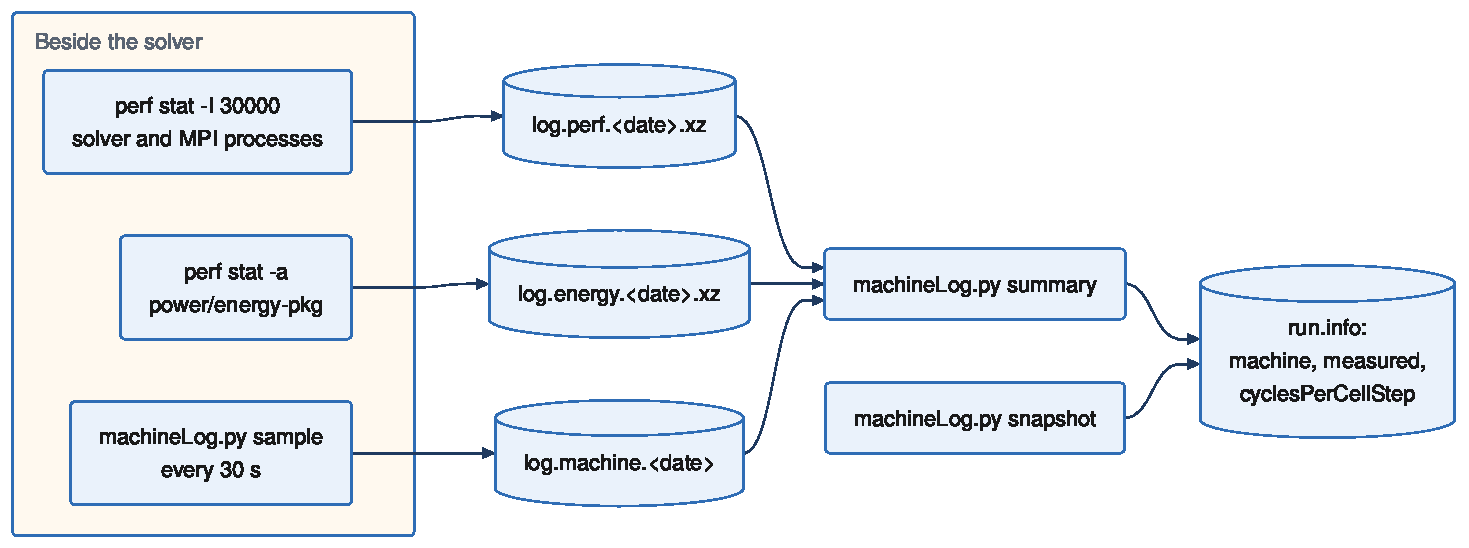
\includegraphics[width=\linewidth]{figures/pdf/measurement.pdf}
  \caption{Measurement during the solver and its record in \texttt{run.info}.}
  \label{fig:measurement}
\end{figure}

\begin{tabularx}{\linewidth}{@{}P{0.26\linewidth} P{0.26\linewidth} L@{}}
\toprule
File & Tool & Contents \\
\midrule
\file{log.perf} & \cmd{perf stat -I 30000} on the solver & Every \unit{30}{s}: task clock, cycles, instructions, front-end stalls, cache misses, migrations, context switches. \\
\file{log.machine} & \file{machineLog.py sample} & Every \unit{30}{s}: wall, monotonic and boot clocks, CPU frequency, load, temperatures of CPU, memory and NVMe, fans, CPU profile. \\
\file{log.energy} & \cmd{perf stat -a -e power/energy-pkg/} & Energy of the CPU package every \unit{30}{s}. Only if \cmd{perf} can count on the whole system. \\
\bottomrule
\end{tabularx}

\begin{longtable}{@{}P{0.32\linewidth} P{0.62\linewidth}@{}}
\caption{Block \texttt{measured} of \texttt{run.info}.}\label{tab:measured}\\
\toprule
Entry & Meaning \\
\midrule
\endfirsthead
\toprule
Entry & Meaning \\
\midrule
\endhead
\ent{suspendedSeconds} & Change of the boot clock minus change of the monotonic clock: the time that the computer was suspended. If it is not 0, the wall time is not a cost. \\
\ent{mhzMean}, \ent{mhzMinOfMean} & Mean clock of all logical CPUs, and the lowest mean of \unit{30}{s}. \\
\ent{tCpuMax}, \ent{tDimm<i>Max}, \ent{tNvmeMax} & Highest temperatures. DDR5 memory doubles its refresh above \unit{85}{\textdegree C}. \\
\ent{profiles} & The CPU profiles during the run. If it is not only \val{performance}, the run does not compare. \\
\ent{cpuSeconds} & CPU time of all solver processes. \\
\ent{cycles}, \ent{instructions} & Totals of all processes. \\
\ent{GHzEffective} & $\text{cycles}/\text{cpuSeconds}$: the real clock of the solver, with turbo and throttling. \\
\ent{IPC} & $\text{instructions}/\text{cycles}$. Low ($\lesssim 1$) in a code that the memory bandwidth limits. \\
\ent{frontendStallFraction} & Cycles with a stopped front end, divided by the cycles. \\
\ent{cacheMisses}, \ent{cpuMigrations}, \ent{contextSwitches} & Indicators of noise. Many migrations show a binding that does not work. \\
\ent{energyPkgJ} & Energy of the CPU package during the solver. \\
\bottomrule
\end{longtable}

The block \ent{machine} gives the state at the start: kernel, sockets, cores, threads
for each core, memory, CPU governor and energy preference, boost, maximum frequency,
CPU profile, fan level, \ent{perf_event_paranoid}, OpenFOAM build and Open MPI version.

\ent{cyclesPerCellStep} is the cost that does not depend on the clock. It includes the
start (the solver reads the mesh), which is small in a run of thousands of steps.

\subsection{Requirements}

\begin{itemize}
\item \ent{kernel.perf_event_paranoid} $\leq 1$ to count the cycles. If not,
  \file{Allrun} shows a message with \val{!!} and runs without \ent{cycles}.
\item $\leq 0$ (or \ent{CAP_PERFMON}) to measure the energy (\cref{sec:prepare-computer}).
\end{itemize}

\subsection{Procedure to get a comparable cost}

\begin{steps}
\item Do the steps of \cref{sec:prepare-computer}.
\item Run one case at a time, with nothing heavy beside it.
\item Use the same number of processes and the same binding for the two solvers: one
  process for each physical core.
\item Before you use the cost of a run, examine \ent{suspendedSeconds},
  \ent{profiles}, \ent{GHzEffective} and \ent{cpuMigrations}.
\end{steps}

\subsection{Do not divide by the clock frequency}

A correction of the wall time by the clock supposes that the time changes as $1/f$.
This is true for a code that the computation limits, not for a code that the memory
bandwidth limits. The two solvers differ in this property: OpenFOAM (low order)
depends more on the memory bandwidth, Nektar++ at a high polynomial order more on the
clock. To measure it, run the same short case at several clock limits
(\ent{scaling_max_freq} at 2, 3 and \unit{4}{GHz}) and fit
\[
  t(f) = t_\text{mem} + \frac{C}{f}.
\]
This procedure is not automated.

\subsection{Runs without this measurement}

The runs before 2026-10-17 have only \file{timeInfo.dat}. An interval with wall time
much larger than CPU time is a suspension. An interval with CPU time much above the
median is a low clock or a load beside the run. Without those intervals, the $h0$ runs
on \texttt{nemepad} cost 20 to 22 core-\textmu s for each cell and step.

\section{Monitor a run}\label{sec:monitor}

\begin{shell}
./post/monitor.sh <run-dir> [seconds]     # default 30 s
\end{shell}

The script plots $C_D$ and $C_L$ against the iteration and the initial residuals on a
logarithmic scale, and draws them again every \val{[seconds]}. It joins the
directories of a continued run. Without a display, it writes
\file{<run-dir>/monitor.png}. It needs \cmd{gnuplot}.

\section{Table of a sweep}\label{sec:sweeptable}

\begin{shell}
./post/sweepTable.sh [runs-dir] > sweep.csv    # default ~/runs
\end{shell}

One line for each run. A run that did not start has empty fields.

\begin{longtable}{@{}P{0.42\linewidth} P{0.52\linewidth}@{}}
\toprule
Columns & Source \\
\midrule
\endhead
\val{case}, \val{mesh}, \val{nCells} & \file{run.info} \\
\val{solver} & \ent{application} in \file{controlDict} \\
\val{Minf}, \val{pInf}, \val{Tinf}, \val{alpha} & \file{flowConditions} \\
\val{status}, \val{steps}, \val{tEnd}, \val{wallSeconds} & Last record of \file{run.info} \\
\val{Cd}, \val{Cl}, \val{CmPitch} & Last line of \file{coefficient.dat} \\
\val{window}, \val{CdMean}, \val{ClMean}, \val{CmPitchMean} & Mean over the window of the stop criterion \\
\val{resUx} \ldots{} \val{resOmega} & Last initial residuals. \val{resP} is empty for \cmd{rhoCentralFoam}. \\
\val{yPlusMin}, \val{yPlusMax}, \val{yPlusAvgWalls}, \val{yPlusAvgFins} & \yplus{} at the last time \\
\bottomrule
\end{longtable}

With a continued run, the coefficients and residuals come from the last start-time
directory only.

\section{Disk}

\begin{itemize}
\item The solver log is compressed with \cmd{xz} at the end. While the solver runs,
  the log grows by 1 to \unit{2}{kB} for each step.
\item \ent{residuals} and the coefficients write one line every 50 steps.
\item \file{constant/polyMesh} is a link to the mesh, except with \ent{--refine}.
\item \ent{purgeWrite 1} keeps only the last time. \file{processor*} is removed when
  \cmd{reconstructPar} ends correctly.
\end{itemize}

\begin{caution}
Many cases link to one mesh. If you remove or make a mesh again, all the cases that
use it lose their mesh.
\end{caution}

\section{Notification}\label{sec:notify}

\file{Allrun} sends a POST request at the end of each run, with the case name,
\val{ok} or \val{failed}, the time, $C_D$ and the hours of wall time. With ntfy, write
the URL of a topic in a file:

\begin{shell}
echo https://ntfy.sh/<topic> > ~/.config/aconcagua/notify
\end{shell}

The topic is public for each person who knows its name: use a name that is difficult
to guess. The environment variable \cmd{NOTIFY_URL} has priority over the file. No
notification comes if \file{runCase.sh} is stopped or if the computer stops.
